\section{Contexto y motivaci�n}

\subsection{Memoria corporativa}
\begin{frame}
	\frametitle{Memoria Corporativa}
	%%%%%%%%%%%%%%%%%%%%%%%
	\begin{block}{Definici�n}
	\justifying 
	La representaci�n expl�cita, t�cita, consistente y persistente del conocimiento de una organizaci�n. \cite{Ontoinra2002}
	\end{block}
	
	\begin{figure}[htbp]
	\centering
	\subfigure{
	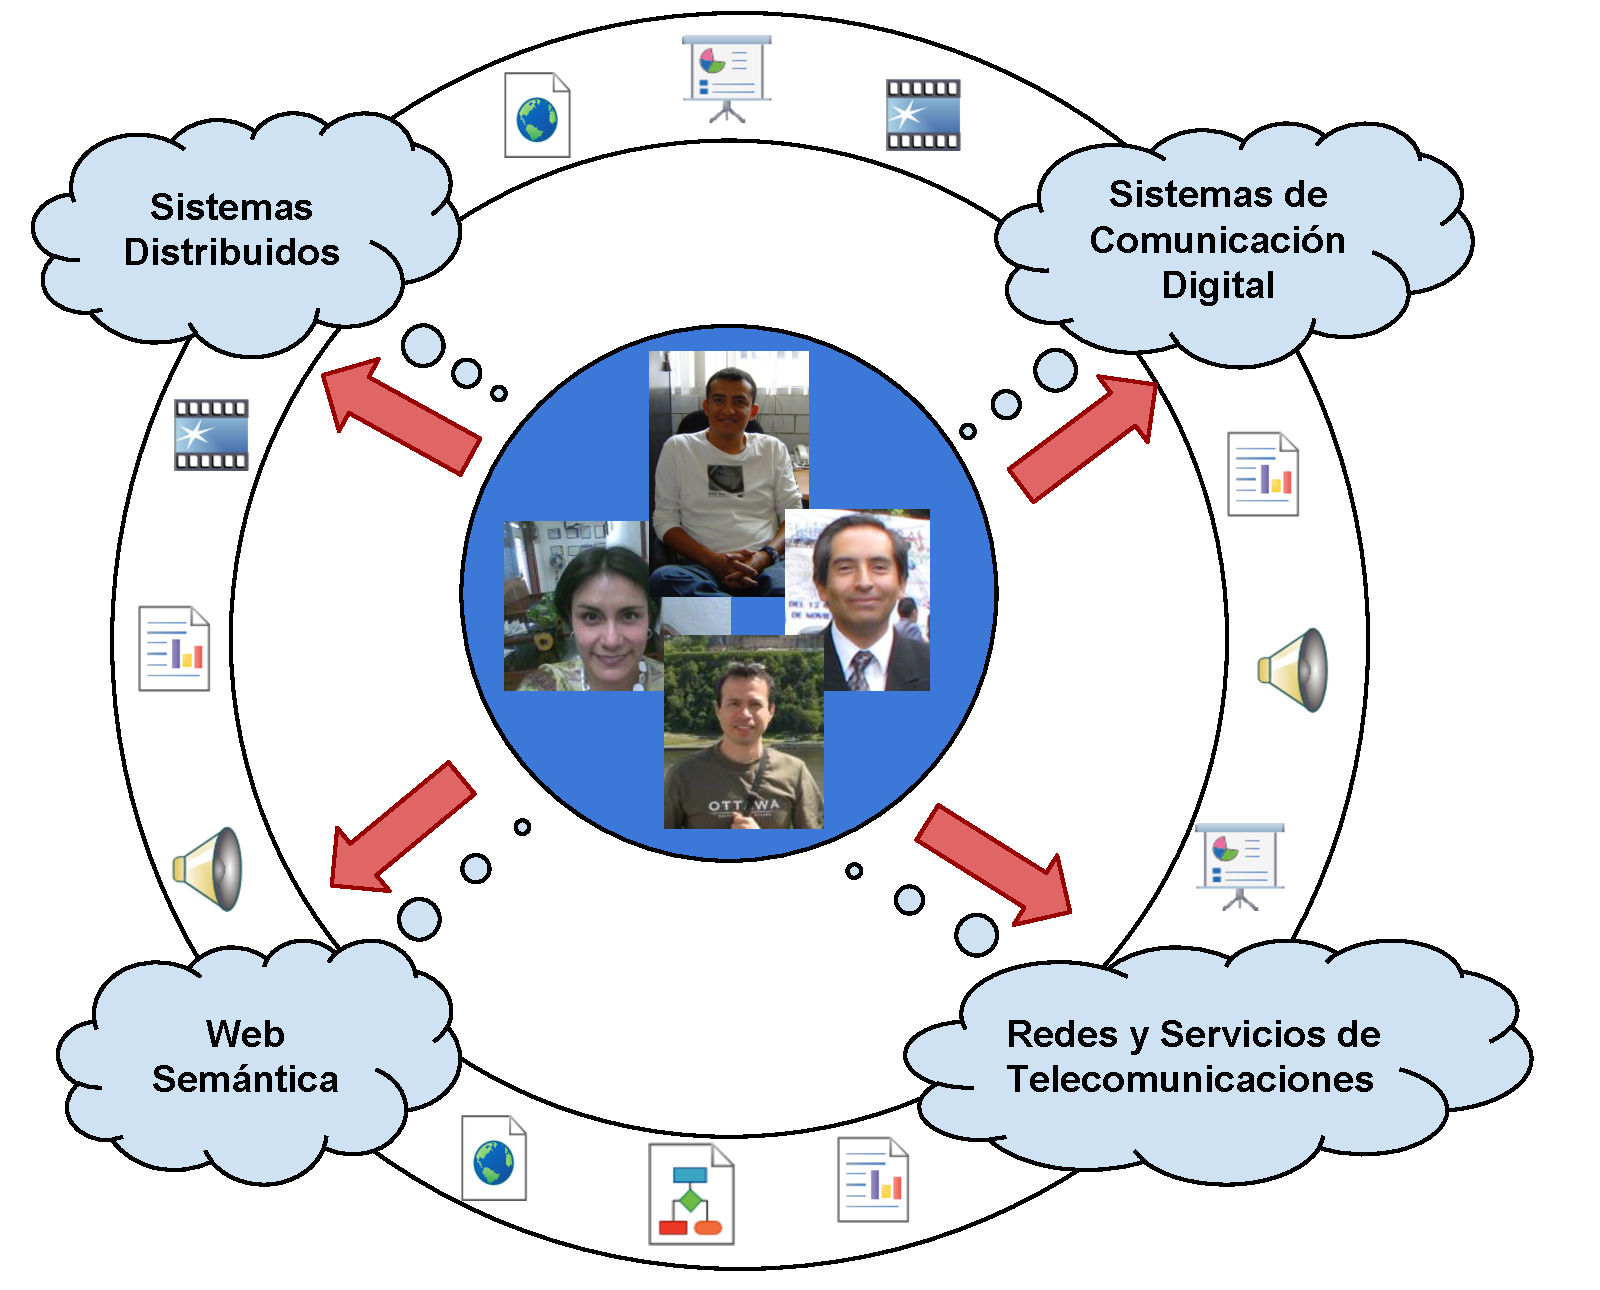
\includegraphics[scale=0.18]{ConocimientoRyT} 
	}
	\subfigure{
	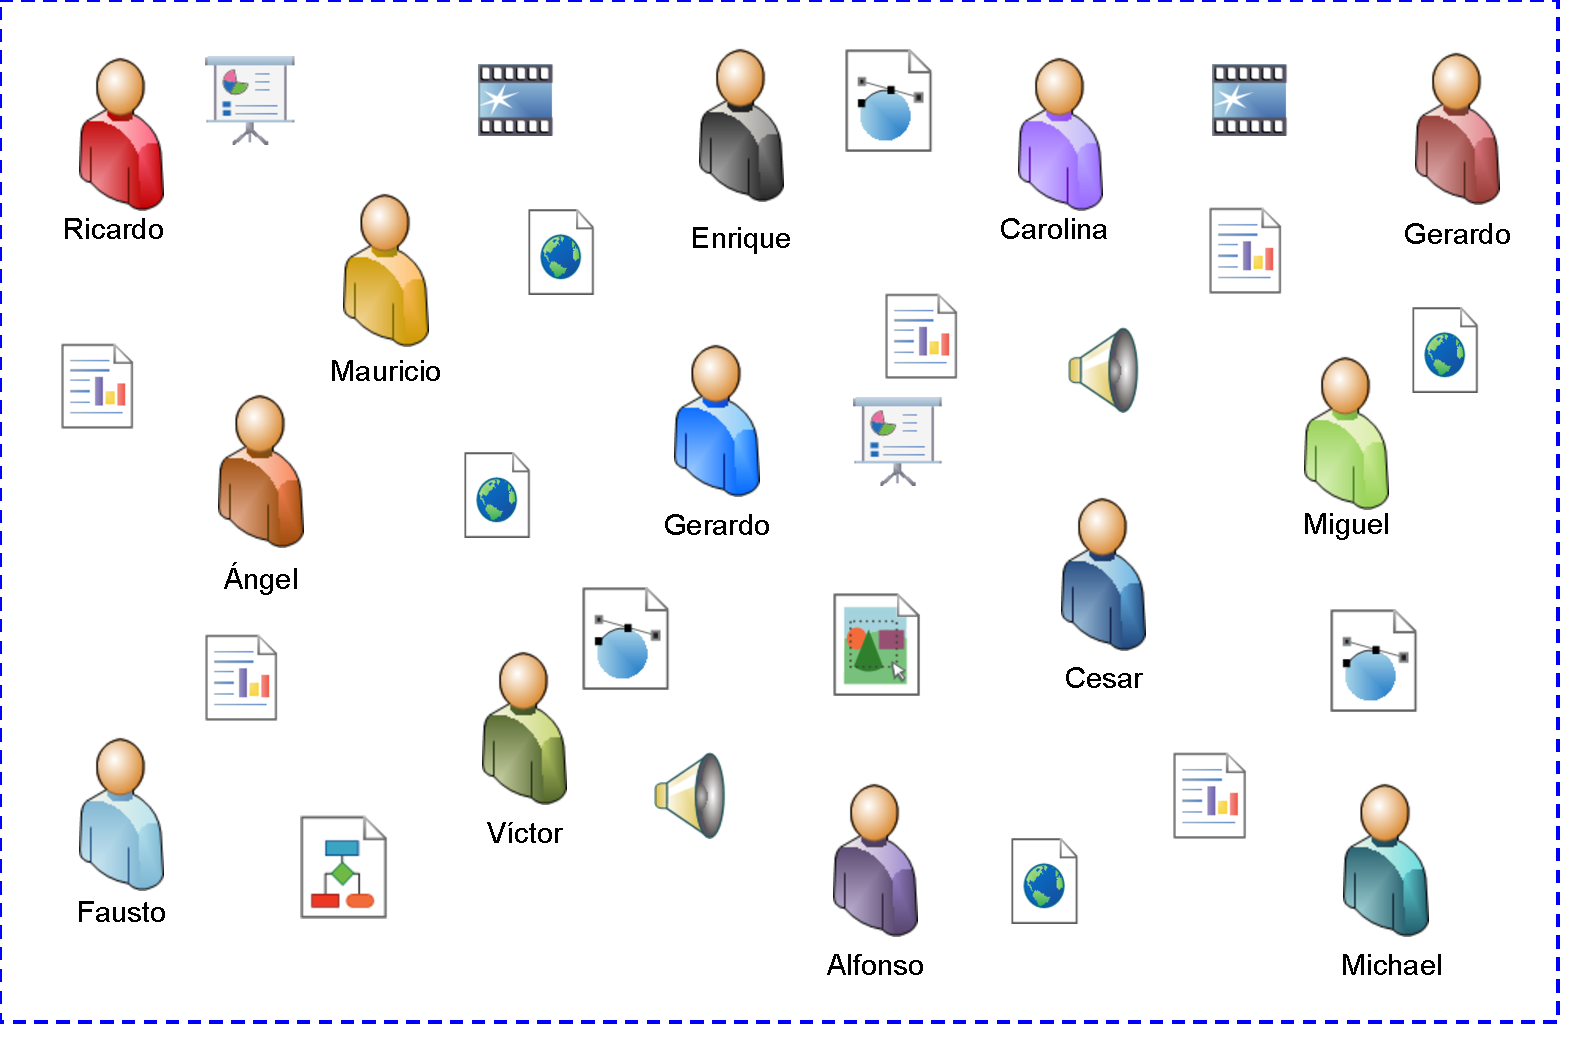
\includegraphics[scale=0.19]{EjemploMC} 
	}
	\end{figure}
	%%%%%%%%%%%%%%%%%%%%%%%
\end{frame}

\subsection{Integraci�n de la informaci�n de los recursos de informaci�n}
\begin{frame}
	\frametitle{Integraci�n de la informaci�n de los recursos de informaci�n}
	\begin{block}{Definici�n}
	\justifying
	\small La b�squeda y recuperaci�n significativa de informaci�n existente en los recursos de informaci�n para responder una consulta dada por un usuario.
	\end{block}
	
	\begin{exampleblock}{Etapas}
	\begin{enumerate}[<+-| alert@+>]
	\item \justifying \small Representar el conocimiento e informaci�n de los \textit{recursos de informaci�n}.
	\item \justifying \small Buscar y recuperar informaci�n, mediante la interrogaci�n de la representaci�n de conocimiento (modelo).
	\end{enumerate}
	\end{exampleblock}
	
	\begin{figure}
	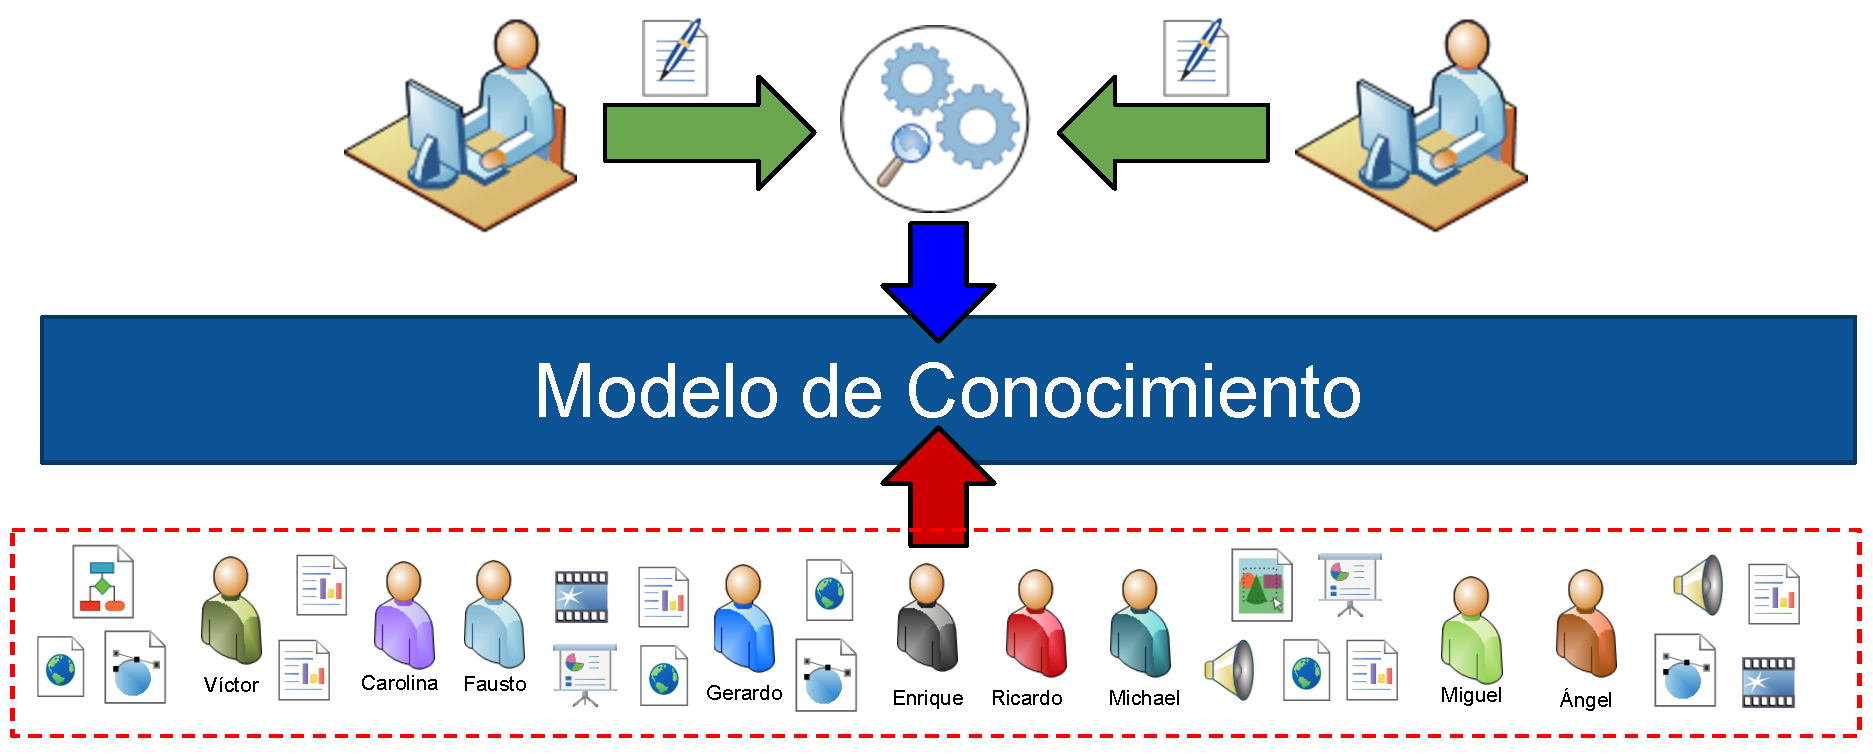
\includegraphics[scale=0.24]{IntegracionSemantica} 
	\end{figure}
\end{frame}

\subsection{Tecnolog�as Sem�nticas}
\begin{frame}
	\frametitle{Tecnolog�as Sem�nticas}
	\begin{block}{Definici�n}
	\justifying 
	\textit{Un conjunto de metodolog�as, lenguajes, aplicaciones, herramientas y est�ndares para suministrar u obtener el significado de las palabras, informaci�n y las relaciones entre �stos}. \begin{scriptsize}\cite{SemTecRetr}\end{scriptsize}
	\end{block}
	
	\begin{figure}
	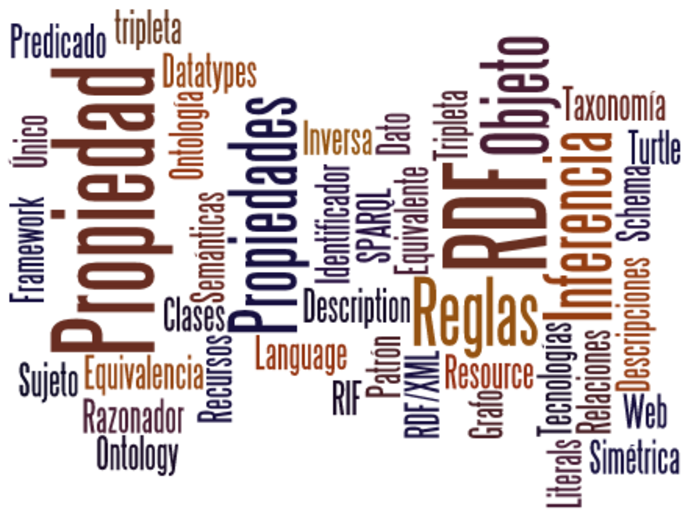
\includegraphics[scale=0.42]{TSWords} 
	\end{figure}
\end{frame}

\subsection{Integraci�n sem�ntica de recursos de informaci�n}
\begin{frame}
	\frametitle{Integraci�n sem�ntica de recursos de informaci�n}
	\begin{figure}
	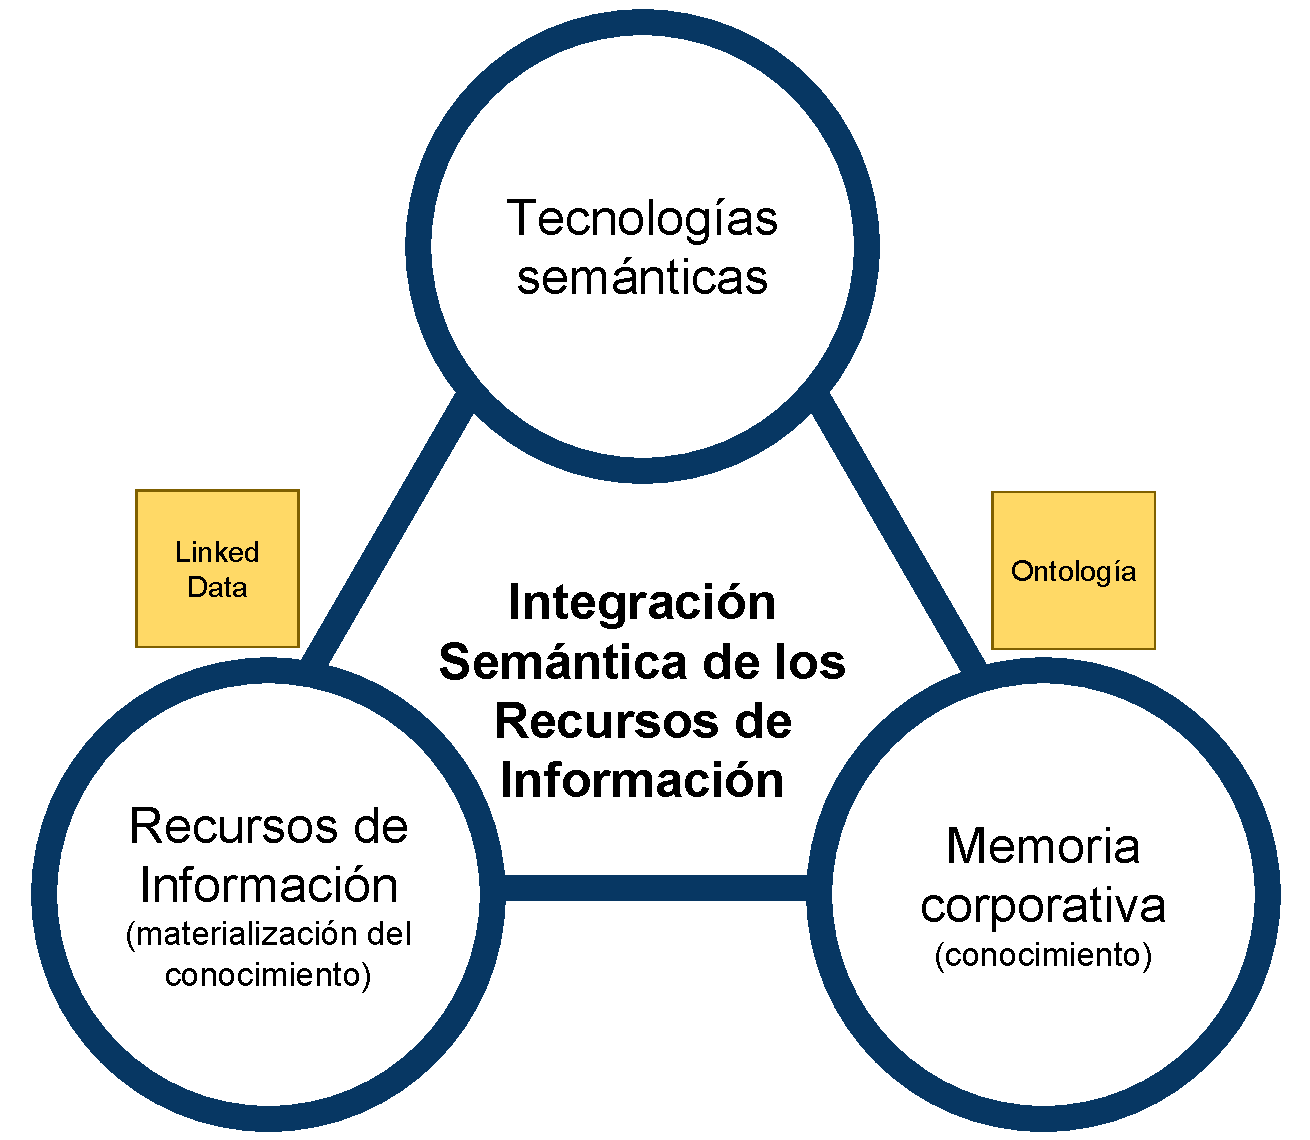
\includegraphics[scale=0.38]{ISRIMC} 
	\end{figure}
\end{frame}

\subsection{Estado del Arte}
\begin{frame}
	\frametitle{Estado del Arte}
	\begin{block}{Ejes claves}
	\begin{enumerate}
	\item \justifying Integraci�n de la informaci�n a partir del uso de tecnolog�as sem�nticas.
	\item \justifying B�squeda, recuperaci�n y publicaci�n de la informaci�n desde una ontolog�a.
	\item \justifying Gesti�n de una memoria corporativa.
	\end{enumerate}
	\end{block}
	
	\begin{figure}
	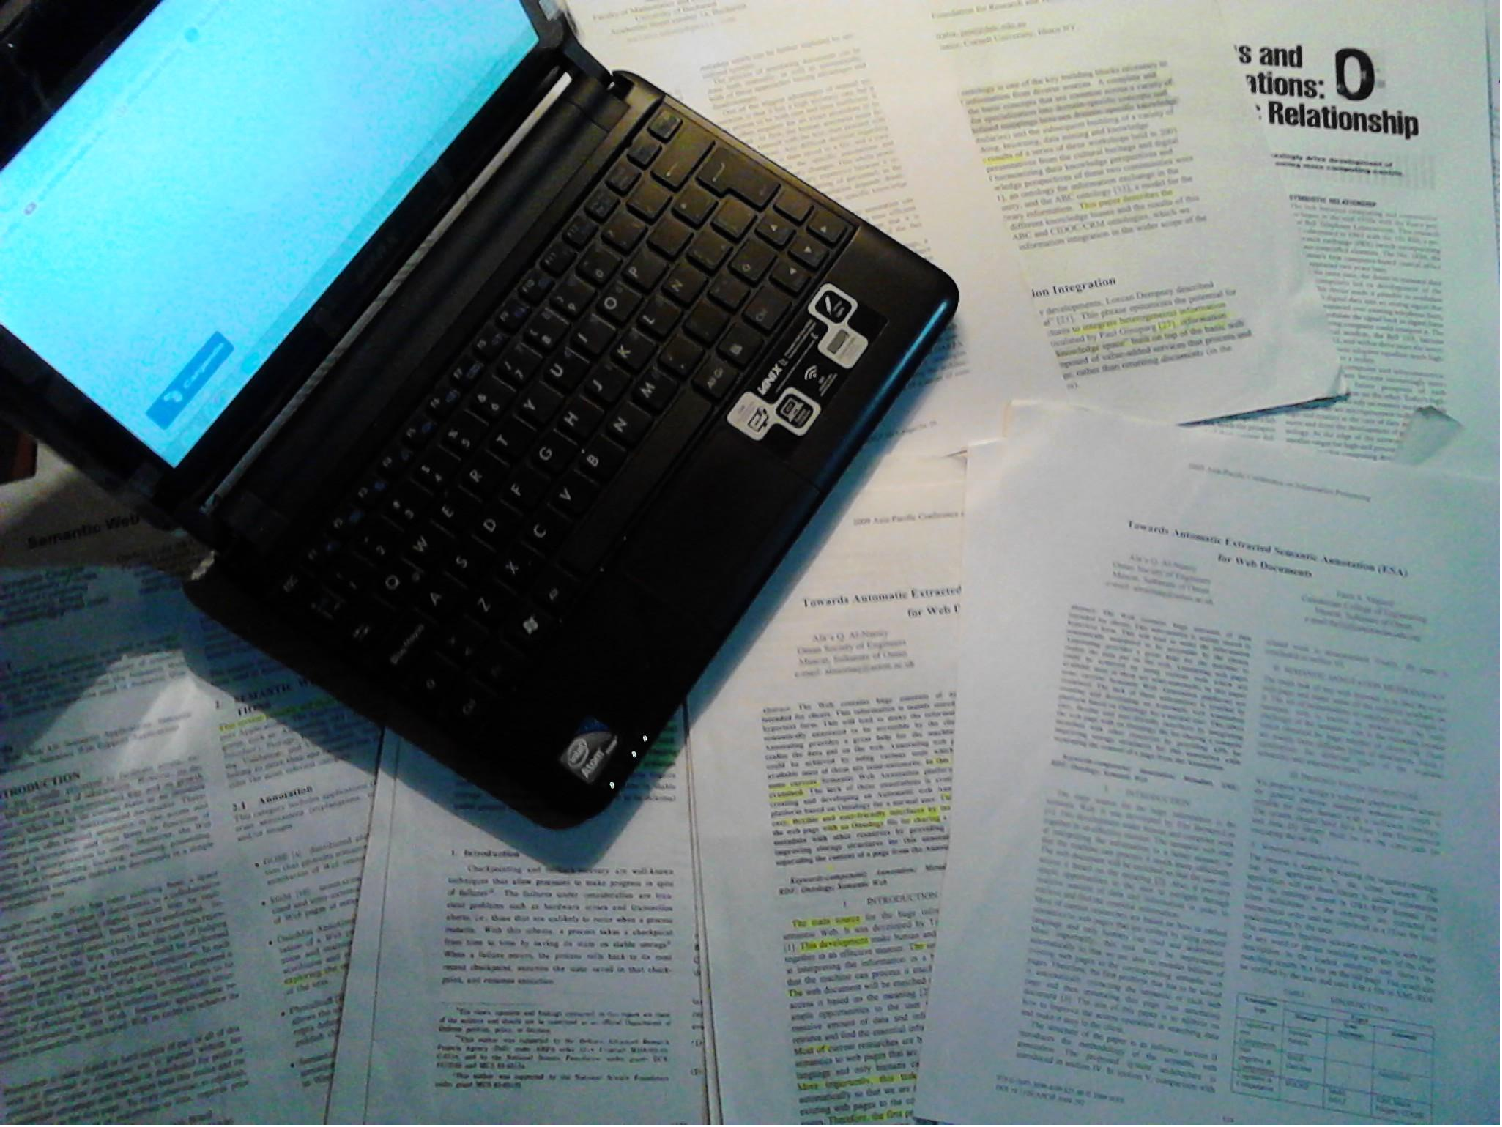
\includegraphics[scale=0.15]{EstadoArte} 
	\end{figure}
\end{frame}

\begin{frame}
	\frametitle{Comparativa}
	\begin{figure}
	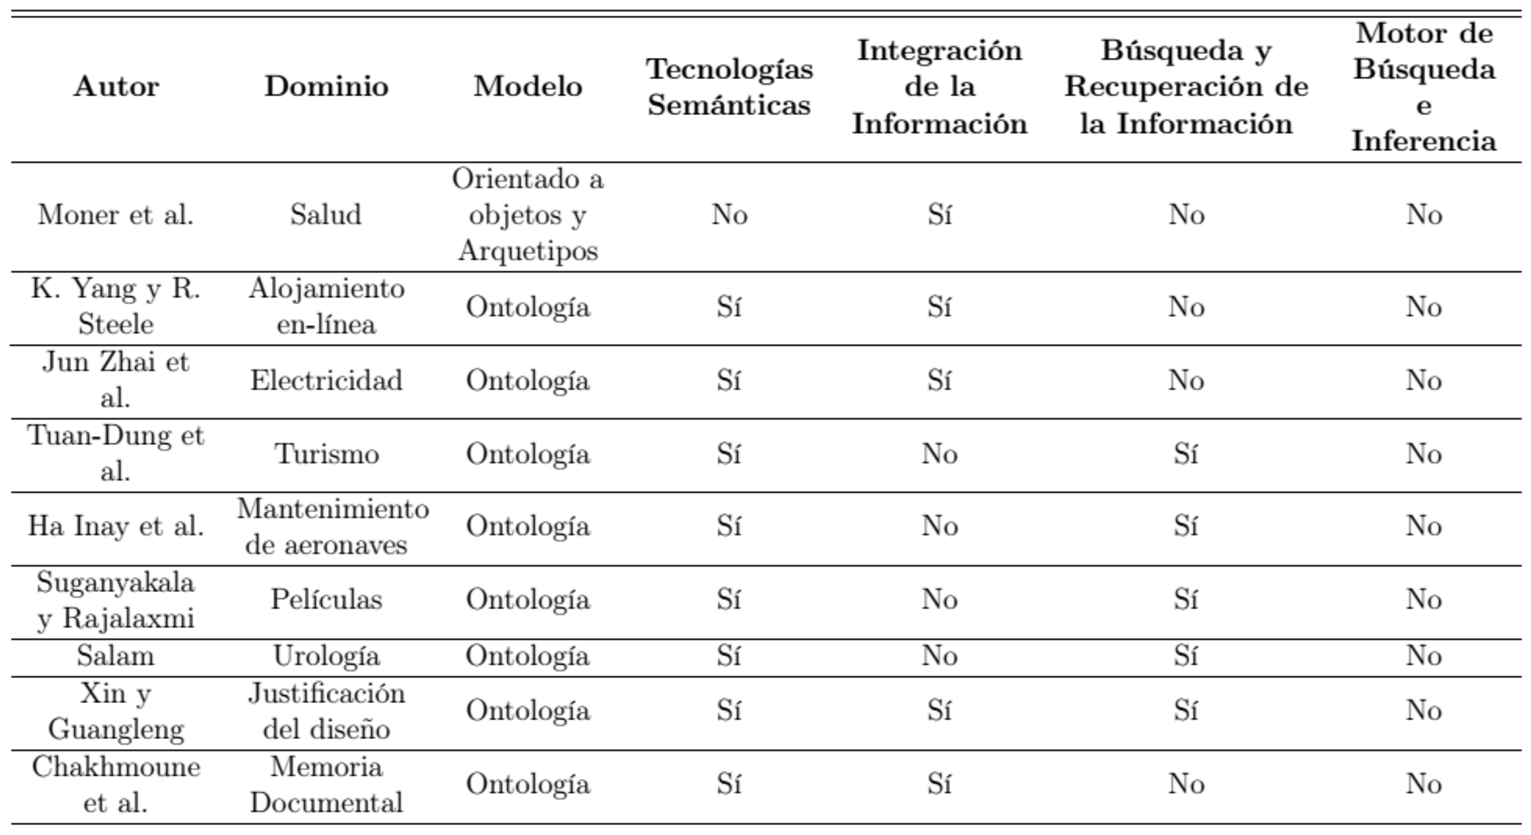
\includegraphics[scale=0.42]{TablaEOA} 
	\end{figure}
\end{frame}